\documentclass[10pt,twocolumn]{jarticle}
% 大阪大学基礎工学部知能システム学コース 特別研究概要スタイルファイル
\typeout{大阪大学基礎工学部知能システム学コース 特別研究概要スタイルファイル(2019/12/24) by 堀井隆斗}

\usepackage{amsmath,amssymb,bm}
\usepackage[dvipdfmx]{graphicx}
%\usepackage[dvips]{graphicx}
\usepackage{ascmac}
\usepackage{calc}
\usepackage{kvsetkeys}
\usepackage{kvoptions}
\usepackage{tikz}
\usepackage{progressbar}
\usepackage{algorithm}
\usepackage{algpseudocode}
\usepackage {subfigmat}
\usepackage {diagbox}
\flushbottom
\sloppy

% 余白

\setlength{\paperwidth}{210mm}
\setlength{\paperheight}{297mm}
\setlength{\voffset}{0mm}
\setlength{\textwidth}{\paperwidth}
\addtolength{\textwidth}{-30mm}
\setlength{\textheight}{\paperheight}
\addtolength{\textheight}{-40mm}
\setlength{\topmargin}{-1in}
\addtolength{\topmargin}{15mm}
\setlength{\headheight}{0mm}
\setlength{\headsep}{0mm}
\setlength{\footskip}{10mm}
\setlength{\oddsidemargin}{-1in}
\addtolength{\oddsidemargin}{15mm}
\setlength{\columnsep}{7mm}

% ヘッダ＆タイトル

\makeatletter
\def\headding#1{\gdef\@headding{#1}}
%\headding{研究進捗報告書}
\def\@maketitle{\newpage
\setlength{\topsep}{0mm}
 \null
 \begin{center}
 {\Large {\bf \@title} \par}
 \vspace{1mm}
 {\large 学籍番号：{\@date} \hspace{10pt} 吉川研究室 \hspace{10pt} {\@author} \par}
 \end{center}
 \vskip 1.5\baselineskip
 }
% 章間の間隔を調整する
\renewcommand{\section}{%
  \@startsection{section}{1}{\z@}%
  {0.4\Cvs}{0.1\Cvs}%
  {\large\bf}}
%  {\normalfont\large\headfont\raggedright}}

\renewcommand{\subsection}{%
  \@startsection{subsection}{1}{\z@}%
  {0.4\Cvs}{0.1\Cvs}%
  {\large\bf}}

\renewcommand{\subsubsection}{%
  \@startsection{subsubsection}{1}{\z@}%
  {0.4\Cvs}{0.1\Cvs}%
  {\normalsize}}
\makeatother

% 図のキャプションをFig.に，表のキャプションをTableにする

\def\fnum@figure{{\bf \figurename}~\thefigure}
\renewcommand{\figurename}{Fig.}

\def\fnum@table{{\bf \tablename~\thetable}}
\renewcommand{\tablename}{Table}

% 箇条書きの行間調節

\renewenvironment{itemize}{%
  \begin{list}{\theenumi.~}{%
  \usecounter{enumi}%
  \setlength{\itemsep}{-.5\baselineskip}%
  \setlength{\parsep}{.5\baselineskip}%
  }}{\end{list}}

% 本文中の数式を別行立て数式と同じように表示する

\everymath{\displaystyle}

\pagestyle{empty} % すべてのページ番号を消

\title{対照学習と強化学習によるオノマトペの歩容スタイル付与}
\date{09C23707} %学籍番号
\author{佐々木條太}

\usepackage[dvipdfmx]{graphicx}
\usepackage[margin=15mm]{geometry}
\usepackage{setspace}
\usepackage{booktabs}

% captionの余白が広すぎるので狭く
\setlength{\abovecaptionskip}{-0.1pt}
\setlength{\belowcaptionskip}{-0.1pt}

\begin{document}
\maketitle
\section{はじめに}
自律移動ロボットのナビゲーション技術はVision-Language-Action（VLA）モデルにより急速に発展している．
しかし，既存のVLAモデルの多くは目的地への到達に主眼を置いており，「どのように移動するか」という移動スタイルの制御は十分に扱われていない．
実環境では効率性だけでなく，静粛性や慎重さ，力強さといった運動の質も重要であり，病院内では静かに振る舞い，急ぐ場面ではきびきびと移動するといった「振る舞いの質感」の制御が求められる．

本研究では，日本語オノマトペ（擬音語・擬態語）を用いて移動スタイルを記述・制御する手法を提案する．
オノマトペは「てくてく」「のっしのっし」「そろりそろり」など短い語句で，速度やリズム，力強さといった多次元的な運動特徴を表現できる．
この性質を活かし，ユーザは指定せずとも感覚的な語彙で運動の質を伝えられる．

%%%%%%%%%%%%%%%%%%%%%%%%%%%%%%%%%%%%%%%%%%%%%%%%%%%%%%%%%%%%%%%%%%%%%%%%%%%%%%%%%%%%%%%%%%%%%%%%%%%%%%%%%%%%%%%%%%%%%%%%%%%%%%%%%%%%%%%%%%%%%%%%%%%%%%%%%%%%%%%%%%%%%%%%%%%%%
\section{提案手法}
提案手法はオフライン対照学習とオンライン強化学習の2段階で構成される（Fig.\ref{fig:overview}）．

\textbf{Phase 1（対照学習）}：
HOYOデータセット\cite{hoyo}の2D歩容系列とオノマトペを用い，MotionCLIP\cite{MotionCLIP}を基盤とした共有潜在空間を構築する．
変分オートエンコーダによる再構成と，教師あり対照学習による意味整合を同時に学習する．
未知語のオノマトペにも対応できるよう，言語と動作の対応関係を汎化することを目的として対照学習を行う．

\textbf{Phase 2（強化学習）}：
物理シミュレータ上のヒューマノイドロボット（H1）に対し，PPOにより歩行方策を学習する．
ロボット動作をHOYO形式の2D系列へリターゲットし，Phase 1のエンコーダで評価した類似度をスタイル報酬として与える．
タスク報酬は安定して歩かせるための報酬であり，
スタイル報酬は動作潜在 $z_{\mathrm{mot},t}$ と教師潜在 $z_{\mathrm{teach}}$ のコサイン類似度で定義する．
$z_{\mathrm{mot},t}$ はロボットの直近 $L$ フレームの2D系列をPhase 1のエンコーダに入力して得た動作埋め込み，
$z_{\mathrm{teach}}$ は目標オノマトペに対応するHOYO教師のmotionの埋め込みである．
\begingroup
  \setlength{\abovedisplayskip}{2pt}
  \setlength{\belowdisplayskip}{2pt}
  \setlength{\abovedisplayshortskip}{2pt}
  \setlength{\belowdisplayshortskip}{2pt}
  \begin{equation}
      r_{\mathrm{style},t} = \cos\!\left(z_{\mathrm{mot},t}, z_{\mathrm{teach}}\right)
  \end{equation}
\endgroup


%%%%%%%%%%%%%%%%%%%%%%%%%%%%%%%%%%%%%%%%%%%%%%%%%%%%%%%%%%%%%%%%%%%%%%%%%%%%%%%%%%%%%%%%%%%%%%%%%%%%%%%%%%%%%%%%%%%%%%%%%%%%%%%%%%%%%%%%%%%%%%%%%%%%%%%%%%%%%%%%%%%%%%%%%%%%%%
\section{実験}
対照学習は11種類のオノマトペラベルを用い，retrieval 指標 avg\_r@1 で評価した．
強化学習はIsaac Lab上のH1に対しPPOで学習し，歩行目標速度は $0.5\,\mathrm{m/s}$ に固定した．
評価はスタイル一致度（cos類似度）と関節誤差（DTW Err），転倒率とした．

\begin{figure}[t]
    \centering
    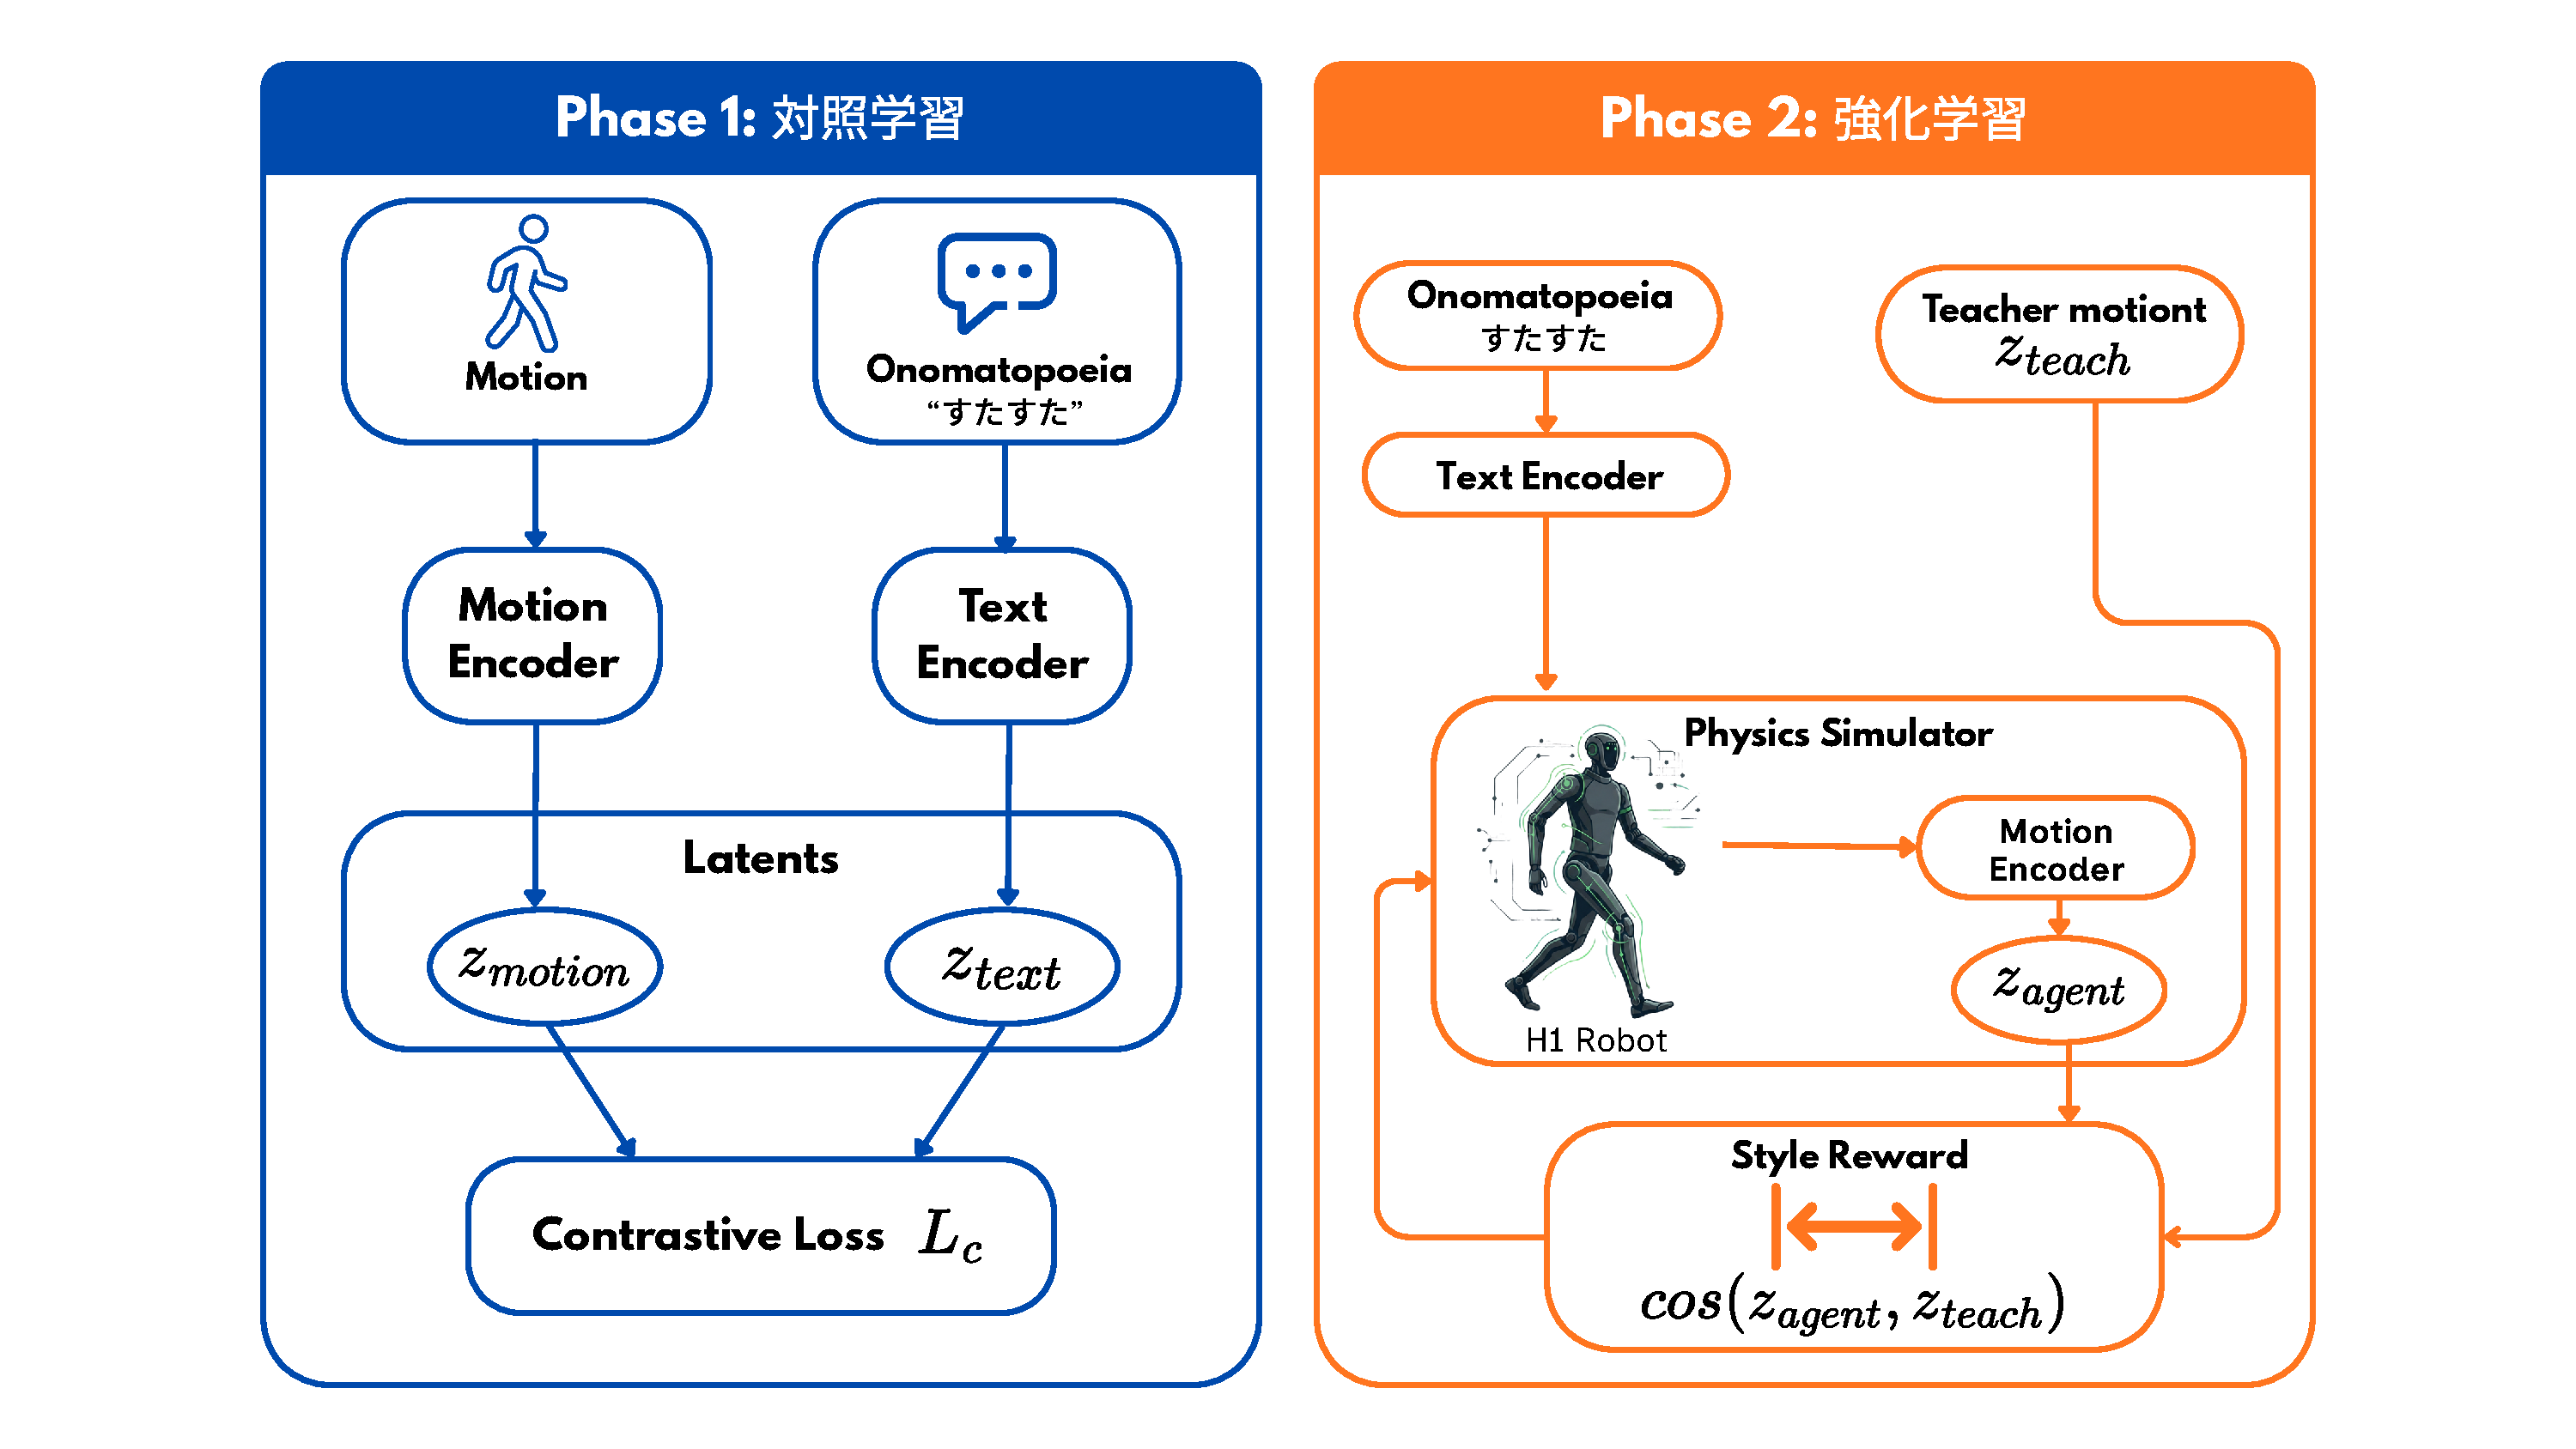
\includegraphics[width=0.85\columnwidth]{fig/Model_Abstract.pdf}
    \caption{提案手法の全体構成（Phase 1: 対照学習／Phase 2: 強化学習）}
    \label{fig:overview}
\end{figure}

\begin{table}[t]
  \centering
  \footnotesize
  \caption{スタイル別の cos 類似度と関節誤差\\
  （歩行目標速度 $0.5\,\mathrm{m/s}$ 固定）}
  \label{tab:rl_cos_err}
  \begin{tabular}{lccc} \toprule
    \textbf{オノマトペ} & 実速度 & Cos類似度 & DTW Err \\ \midrule
    通常         & 0.253 & 0.487 & 4.2928 \\
    すたすた     & 0.318 & 0.527 & 3.9590 \\
    のろのろ     & 0.273 & 0.400 & 4.1939 \\
    どっしどっし & 0.243 & 0.514 & 4.1986 \\
    ぶらぶら     & 0.292 & 0.526 & 4.3407 \\ \bottomrule
  \end{tabular}
\end{table}


\section{結果、考察}
\textbf{対照学習}：
$\mathrm{avg\_r@1}=0.356\pm0.224$ を得た．
VAE 正則化は過学習を抑制する一方で，過度に強い場合は retrieval 性能が下がる傾向が見られた．
未知語を潜在空間で可視化すると，意味的に近い学習ラベルの近傍に配置され，言語—動作対応の汎化獲得が示唆された．

\textbf{強化学習}：
スタイル別の評価結果を Table~\ref{tab:rl_cos_err} に示す．ここで「通常」は，特別なスタイルを付与していない歩行状態を指す．
実速度は入力 $0.5\,\mathrm{m/s}$ に対し $0.243$--$0.318\,\mathrm{m/s}$ とばらつき，
「どっしどっし」「のろのろ」が低速，\,「すたすた」が高速となり，\,オノマトペの印象に沿った傾向が得られた．
cos 類似度は最大 0.527 であり，スタイル追従の余地が残る．
また、ロボットの動作を見ると、腕の動作が崩れていることがあり，姿勢の改善が今後の課題である．


%%%%%%%%%%%%%%%%%%%%%%%%%%%%%%%%%%%%%%%%%%%%%%%%%%%%%%%%%%%%%%%%%%%%%%%%%%%%%%%%%%%%%%%%%%%%%%%%%%%%%%%%%%%%%%%%%%%%%%%%%%%%%%%%%%%%%%%%%%%%%%%%%%%%%%%%%%%%%%%%%%%%%%%%%%%%%%
\section{おわりに}
本研究では，オノマトペを用いてロボットの歩行スタイルを制御する手法を提案した．
対照学習により言語と動作の共有潜在空間を構築し，未知語への汎化性能を確認した．
今後の課題として，実機への適用が挙げられる．
% \addcontentsline{toc}{chapter}{\bibname}
\begin{spacing}{0.9}
\bibliographystyle{junsrt-etal}
\bibliography{references.bib}
\end{spacing}
\end{document}
